% 3D complete heat path (TikZ): top/mid dies (TSV inter-layer) ->
% (ubump) -> interposer -> (C4) -> substrate -> ambient, plus the heatsink
% branch die_top ->(TIM)-> heatsink ->(convection)-> ambient. Both cooling
% paths coexist; branch colors: amber = heatsink, blue = substrate path.
% Physical layers (TSV/ubump/C4/TIM) labeled as chain segments; every
% branch carries physical path type + value provenance; nodes carry
% role/size. All routing orthogonal; sans-serif.
%
% Sources: config/thermal/3d-two-die-explicit.yaml (R_tsv = r_via/n_vias
% = 5 K/W, r_vert = 1.0 K/W top-layer), 2p5d-two-die-heatsink-explicit
% .yaml (r_tim = 0.3 K/W, h*A), thermal-module-catalog formulas for the
% per-segment decomposition; per-segment values not fabricated.
\documentclass[border=10pt]{standalone}
\usepackage{sfmath}
\renewcommand{\familydefault}{\sfdefault}
\usepackage{tikz}
\usetikzlibrary{arrows.meta, shapes.geometric}
\definecolor{diefill}{HTML}{E8F0FE}
\definecolor{dieedge}{HTML}{1A73E8}
\definecolor{ipfill}{HTML}{F3E8FD}
\definecolor{ipedge}{HTML}{9334E6}
\definecolor{subfill}{HTML}{FFF4E5}
\definecolor{subedge}{HTML}{B45309}
\definecolor{pcbfill}{HTML}{E6F4EA}
\definecolor{pcbedge}{HTML}{188038}
\definecolor{hsfill}{HTML}{E0F2F1}
\definecolor{hsedge}{HTML}{00695C}
\definecolor{bndfill}{HTML}{F1F3F4}
\definecolor{bndedge}{HTML}{5F6368}
\definecolor{segsub}{HTML}{1A73E8}
\definecolor{seghs}{HTML}{B45309}
\begin{document}
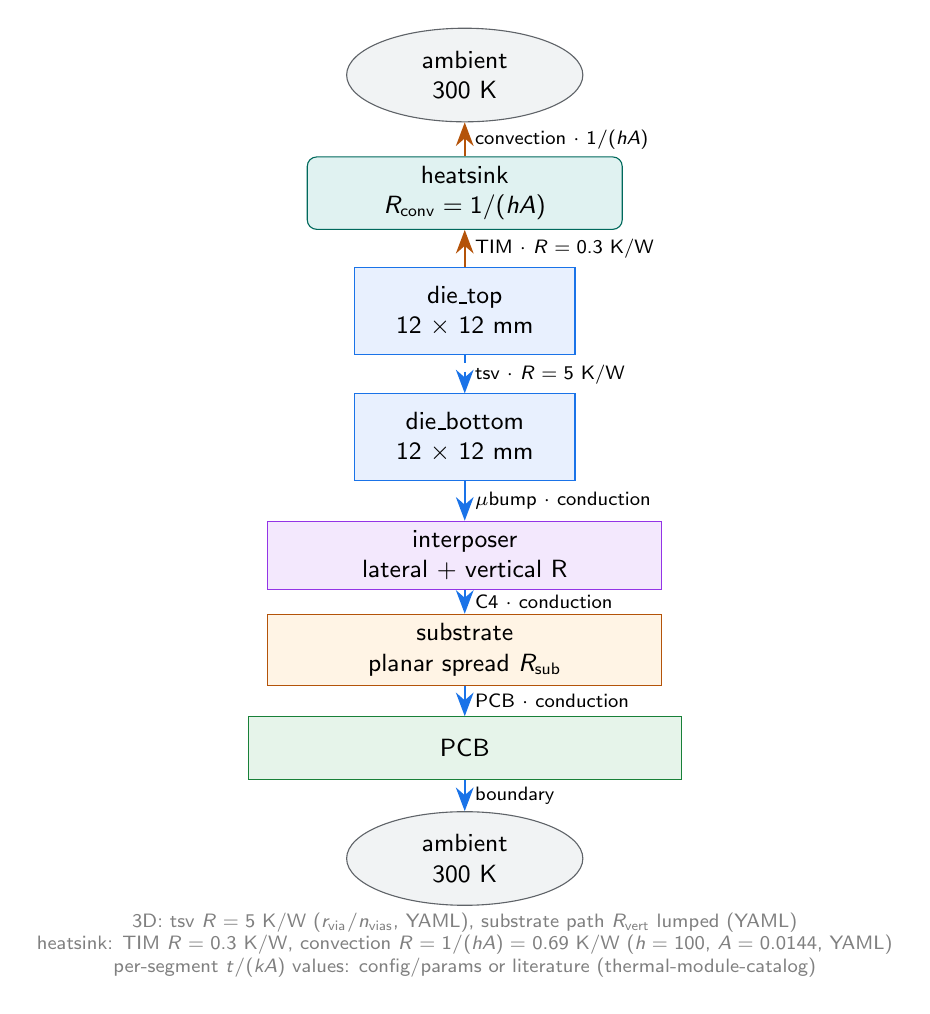
\begin{tikzpicture}[
  die/.style={rectangle, draw=dieedge, fill=diefill, minimum width=2.8cm,
              minimum height=1.1cm, align=center, font=\small},
  layer/.style 2 args={rectangle, draw=#1, fill=#2, minimum width=5.0cm,
              minimum height=0.8cm, align=center, font=\small},
  hs/.style={rectangle, rounded corners=0.12cm, draw=hsedge, fill=hsfill,
             minimum width=4.0cm, minimum height=0.8cm, align=center, font=\small},
  bnd/.style={ellipse, draw=bndedge, fill=bndfill, minimum width=3.0cm,
              minimum height=1.0cm, align=center, font=\small},
  segsub/.style={draw=segsub, thick, -{Stealth[length=3mm]}, rounded corners=0.08cm},
  seghs/.style={draw=seghs, thick, -{Stealth[length=3mm]}, rounded corners=0.08cm},
  tsv/.style={draw=segsub, thick, dashed, -{Stealth[length=3mm]}},
  lab/.style={font=\scriptsize},
]
% ---- stacked dies: top / mid with TSV inter-layer, then substrate path (blue)
\node[die] (die_top) at (0, 2.0) {die\_top\\12 $\times$ 12 mm};
\node[die] (die_bottom) at (0, 0.4) {die\_bottom\\12 $\times$ 12 mm};
\node[layer={ipedge}{ipfill}] (interposer) at (0, -1.1) {interposer\\lateral + vertical R};
\node[layer={subedge}{subfill}] (substrate) at (0, -2.3) {substrate\\planar spread $R_{\mathrm{sub}}$};
\node[layer={pcbedge}{pcbfill}, minimum width=5.5cm] (pcb) at (0, -3.55) {PCB};
\node[bnd] (ambient) at (0, -4.95) {ambient\\300 K};
\draw[tsv] (die_top.south) -- node[right, lab] {tsv $\cdot$ $R=5$ K/W} (die_bottom.north);
\draw[segsub] (die_bottom.south) -- node[right, lab] {$\mu$bump $\cdot$ conduction} (interposer.north);
\draw[segsub] (interposer.south) -- node[right, lab] {C4 $\cdot$ conduction} (substrate.north);
\draw[segsub] (substrate.south) -- node[right, lab] {PCB $\cdot$ conduction} (pcb.north);
\draw[segsub] (pcb.south) -- node[right, lab] {boundary} (ambient.north);
% ---- heatsink branch (amber): die_top -> TIM -> heatsink -> convection -> ambient
\node[hs] (heatsink) at (0, 3.5) {heatsink\\$R_{\mathrm{conv}}=1/(hA)$};
\node[bnd] (ambient_hs) at (0, 5.0) {ambient\\300 K};
\draw[seghs] (die_top.north) -- node[right, lab] {TIM $\cdot$ $R=0.3$ K/W} (heatsink.south);
\draw[seghs] (heatsink.north) -- node[right, lab] {convection $\cdot$ $1/(hA)$} (ambient_hs.south);
% branch annotation: physical path type + value provenance (3 lines)
\node[lab, align=center, text=gray] at (0, -6.05) {
  3D: tsv $R=5$ K/W ($r_{\mathrm{via}}/n_{\mathrm{vias}}$, YAML), substrate path $R_{\mathrm{vert}}$ lumped (YAML)\\
  heatsink: TIM $R=0.3$ K/W, convection $R=1/(hA)=0.69$ K/W ($h=100$, $A=0.0144$, YAML)\\
  per-segment $t/(kA)$ values: config/params or literature (thermal-module-catalog)};
\end{tikzpicture}
\end{document}
